\documentclass[english,11pt,table,handout]{beamer}

% Copyright 2007 by Till Tantau
%
% This file may be distributed and/or modified
%
% 1. under the LaTeX Project Public License and/or
% 2. under the GNU Public License.
%
% See the file doc/licenses/LICENSE for more details.


% Common packages
\usepackage[utf8x]{inputenc}
\usepackage[vietnam,english]{babel}
\usepackage[utf8]{vietnam}
%\usepackage{times}
\usefonttheme[onlymath]{serif}
\usecolortheme{default}
\usepackage{booktabs}
\usepackage{mathpartir}
\usepackage{listings}
\usepackage{listingsutf8}

\usepackage{pbox}
\mprset{flushleft}
\mode<article>
{
  \usepackage{times}
  \usepackage{mathptmx}
  \usepackage[left=1.5cm,right=6cm,top=1.5cm,bottom=3cm]{geometry}
}

\usepackage{hyperref}
\usepackage{tikz}
\usetikzlibrary{arrows,backgrounds}
%\tikzstyle{mnode}=[circle, draw, fill=black, inner sep=0pt, minimum width=4pt]
\usepackage{colortbl}
%\usepackage{yfonts}
\usepackage{translator} % comment this, if not available


% Common settings for all lectures in this course

\def\lecturename{Image Processing and Computer Vision}

\title{\insertlecture}

\author{\textbf{LE Thanh Sach}}

\institute
{
  \textit{Faculty of Computer Science and Engineering}\\
  \textit{Ho Chi Minh University of Technology, VNU-HCM}
}

\subject{Lecturer \lecturename}

% Beamer version theme settings

\useoutertheme[height=0pt,width=2cm,right]{sidebar}
\usecolortheme{rose,sidebartab}
\useinnertheme{circles}
\usefonttheme[only large]{structurebold}

\setbeamercolor{sidebar right}{bg=black!15}
\setbeamercolor{structure}{fg=blue}
\setbeamercolor{author}{parent=structure}

\setbeamerfont{title}{series=\normalfont,size=\LARGE}
\setbeamerfont{title in sidebar}{series=\bfseries}
\setbeamerfont{author in sidebar}{series=\bfseries}
\setbeamerfont*{item}{series=}
\setbeamerfont{frametitle}{size=}
\setbeamerfont{block title}{size=\small}
\setbeamerfont{subtitle}{size=\normalsize,series=\normalfont}

\setbeamertemplate{navigation symbols}{}
\setbeamertemplate{bibliography item}[book]
\setbeamertemplate{sidebar right}
{
  {\usebeamerfont{title in sidebar}%
    \vskip1.5em%
    \hskip3pt%
    \usebeamercolor[fg]{title in sidebar}%
    \insertshorttitle[width=2cm,center,respectlinebreaks]\par%
    \vskip1.25em%
  }%
  {%
    \hskip3pt%
    \usebeamercolor[fg]{author in sidebar}%
    \usebeamerfont{author in sidebar}%
    \insertshortauthor[width=2cm,center,respectlinebreaks]\par%
    \vskip1.25em%
  }%
  \hbox to2cm{\hss\insertlogo\hss}
  \vskip1.25em%
  \insertverticalnavigation{2cm}%
  \vfill
  \hbox to 2cm{\hfill\usebeamerfont{subsection in
      sidebar}\strut\usebeamercolor[fg]{subsection in
      sidebar}\insertshortlecture.\insertframenumber\hskip5pt}%
  \vskip3pt%
}%

\setbeamertemplate{title page}
{
  \vbox{}
  \vskip1em
  {\huge Chapter \insertshortlecture\par}
  {\usebeamercolor[fg]{title}\usebeamerfont{title}\inserttitle\par}%
  \ifx\insertsubtitle\@empty%
  \else%
    \vskip0.25em%
    {\usebeamerfont{subtitle}\usebeamercolor[fg]{subtitle}\insertsubtitle\par}%
  \fi%     
  \vskip1em\par
  \emph{\lecturename}\ 
  %on \insertdate\par
  \vskip3em\par

  \leftskip=0pt plus1fill\insertauthor\par
  \insertinstitute\vskip1em
}

\logo{
\includegraphics[width=1.5cm]{hcmut.png}}



% Article version layout settings

\mode<article>

\makeatletter
\def\@listI{\leftmargin\leftmargini
  \parsep 0pt
  \topsep 5\p@   \@plus3\p@ \@minus5\p@
  \itemsep0pt}
\let\@listi=\@listI


\setbeamertemplate{frametitle}{\paragraph*{\insertframetitle\
    \ \small\insertframesubtitle}\ \par
}
\setbeamertemplate{frame end}{%
  \marginpar{\scriptsize\hbox to 1cm{\sffamily%
      \hfill\strut\insertshortlecture.\insertframenumber}\hrule height .2pt}}
\setlength{\marginparwidth}{1cm}
\setlength{\marginparsep}{4.5cm}

\def\@maketitle{\makechapter}

\def\makechapter{
  \newpage
  \null
  \vskip 2em%
  {%
    \parindent=0pt
    \raggedright
    \sffamily
    \vskip8pt
    {\fontsize{36pt}{36pt}\selectfont Chapter \insertshortlecture \par\vskip2pt}
    {\fontsize{24pt}{28pt}\selectfont \color{blue!50!black} \insertlecture\par\vskip4pt}
    {\Large\selectfont \color{blue!50!black} \insertsubtitle\par}
    \vskip10pt

    \normalsize\selectfont Print version of
    Lecturer \emph{\lecturename} of \@date\par\vskip1.5em
    %\hfill Le Thanh Sach and Luong The Nhan, Faculty of CSE, HCMC University of Technology
  }
  \par
  \vskip 1.5em%
}

\let\origstartsection=\@startsection
\def\@startsection#1#2#3#4#5#6{%
  \origstartsection{#1}{#2}{#3}{#4}{#5}{#6\normalfont\sffamily\color{blue!50!black}\selectfont}}

\makeatother

\mode
<all>




% Typesetting Listings

\usepackage{listings}
\lstset{language=Java}

\alt<presentation>
{\lstset{%
  basicstyle=\footnotesize\ttfamily,
  commentstyle=\slshape\color{green!50!black},
  keywordstyle=\bfseries\color{blue!50!black},
  identifierstyle=\color{blue},
  stringstyle=\color{orange},
  escapechar=\#,
  emphstyle=\color{red}}
}
{
  \lstset{%
    basicstyle=\ttfamily,
    keywordstyle=\bfseries,
    commentstyle=\itshape,
    escapechar=\#,
    emphstyle=\bfseries\color{red}
  }
}



% Common theorem-like environments

\theoremstyle{example}
\newtheorem{exercise}[theorem]{\translate{Exercise}}


% New useful definitions:

\newbox\mytempbox
\newdimen\mytempdimen

\newcommand\includegraphicscopyright[3][]{%
  \leavevmode\vbox{\vskip3pt\raggedright\setbox\mytempbox=\hbox{\includegraphics[#1]{#2}}%
    \mytempdimen=\wd\mytempbox\box\mytempbox\par\vskip1pt%
    \fontsize{3}{3.5}\selectfont{\color{black!25}{\vbox{\hsize=\mytempdimen#3}}}\vskip3pt%
}}

\newenvironment{colortabular}[1]{\medskip\rowcolors[]{1}{blue!20}{blue!10}\tabular{#1}\rowcolor{blue!40}}{\endtabular\medskip}

\def\equad{\leavevmode\hbox{}\quad}

\newenvironment{greencolortabular}[1]
{\medskip\rowcolors[]{1}{green!50!black!20}{green!50!black!10}%
  \tabular{#1}\rowcolor{green!50!black!40}}%
{\endtabular\medskip}
\usepackage{pgf}

\newcommand{\Rule}[2]{\genfrac{}{}{0.7pt}{}{{\setlength{\fboxrule}{0pt}\setlength{\fboxsep}{3mm}\fbox{$#1$}}}{{\setlength{\fboxrule}{0pt}\setlength{\fboxsep}{3mm}\fbox{$#2$}}}}

\newcommand{\Rulee}[3]{\genfrac{}{}{0.7pt}{}{{\setlength{\fboxrule}{0pt}\setlength{\fboxsep}{3mm}\fbox{$#1$}}}{{\setlength{\fboxrule}{0pt}\setlength{\fboxsep}{3mm}\fbox{$#2$}}}[#3]}

\usepackage{url}

\usepackage{qtree}

\usepackage{datetime}

\usepackage{amsfonts}
\usepackage{mathtools}
\usepackage{fancybox}
\usepackage[linesnumbered]{algorithm2e}
\usepackage{ragged2e}
\usepackage{verbatim}

\lecture[3]{Image Derivatives}{lecture-text}

% \subtitle{Sequence Control}

\date{09 September 2015}
\newcounter{saveenumi}

\usepackage{wrapfig}
\usetikzlibrary{automata,arrows,positioning, chains, shapes.callouts, calc}

\tikzstyle{mnode}=[circle, draw, fill=black, inner sep=0pt, minimum width=4pt]
\tikzstyle{thinking} = [draw=blue, very thick]
\edef\sizetape{1cm}
\tikzstyle{tmtape}=[draw,minimum size=\sizetape]
\tikzstyle{tmhead}=[arrow box,draw,minimum size=.5cm,arrow box
arrows={east:.25cm, west:0.25cm}]
\tikzset{
  level/.style   = { ultra thick, blue },
  connect/.style = { dashed, red },
  notice/.style  = { draw, rectangle callout, callout relative pointer={#1} },
  label/.style   = { text width=4cm }
}

\begin{document}

\begin{frame}
\selectlanguage{english}
  \maketitle
\end{frame}

\begin{frame}\frametitle<presentation>{Overview}
  \tableofcontents
\end{frame}

%%%%%%%%%%%%%%%%%%%%%%%%%%%%%%%%%%%%%%%%%%%%%%%%%%%%%%%%%%%%%%%%%%%%%
%%%%%%%%%%%%%%%%%%%%%%%%%%%%%%%%%%%%%%%%%%%%%%%%%%%%%%%%%%%%%%%%%%%%%


%\frame
%{
%	\Huge
%	\begin{center}
%	\textcolor{blue}{\textbf{What is local processing?}}
%	\end{center}
%}

\section{Image model}
\frame
{
	\frametitle{Image Model}
	\selectlanguage{english}
	\begin{block}{Image model}
		\begin{itemize}
			\item Image is a function of two variables $x$ and $y$: $f(x,y)$
			\item It can seen as a surface on 2D-space.
		\end{itemize}
	\end{block}
	\begin{figure}[!h]
		\begin{tabular}{cc}
			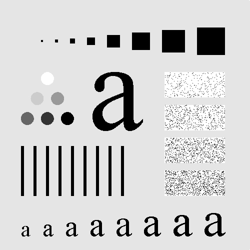
\includegraphics[scale=0.5]{char.png} &
			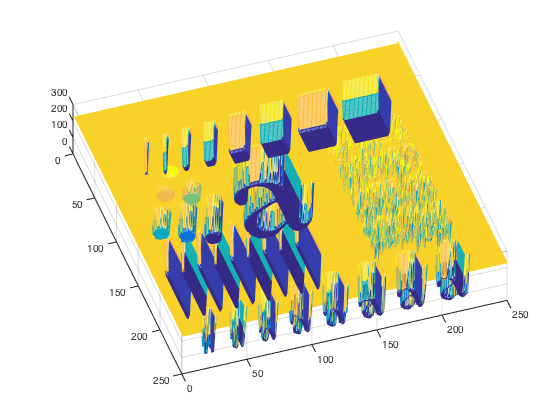
\includegraphics[scale=0.25]{char_mesh.png} \\
			An gray image & Mesh model of the image
		\end{tabular}
		
	\end{figure}
	
}
\section{First-order derivative}
\frame
{
	\frametitle{Derivative of one variable function}
	\selectlanguage{english}
	Taylor expansion for $f(x + \Delta x)$:

	\begin{align} 
	\label{taylor_right}
	f(x + \Delta x) &= f(x) + \Delta x \times f^{'}(x) +\frac{{\Delta x}^2}{2!} \times f^{''}(x) + O({\Delta x}^3) 
	\end{align}

	
	\begin{block}{First-order derivative from Eq. (\ref{taylor_right})}
		\alert{\textbf{Forward Approximation:}} 
		\begin{equation*} 
		\begin{split}
		f^{'}(x) &\cong \frac{f(x+ \Delta x) - f(x)}{\Delta x}\\
				&\cong f(x+1) - f(x) \quad \text{\alert{\textbf{in discrete domain}}}
		\end{split}
		\end{equation*}
		\begin{itemize}
			\item This approximation has error $O({\Delta x})$ 
		\end{itemize}
	\end{block}
	
}
\frame
{
	\frametitle{Derivative of one variable function}
	\selectlanguage{english}
	Taylor expansion for $f(x - \Delta x)$:
	
	
	\begin{align}
	\label{taylor_left}
	f(x - \Delta x) &= f(x) - \Delta x \times f^{'}(x) +\frac{{\Delta x}^2}{2!} \times f^{''}(x) - O({\Delta x}^3) 
	\end{align}
	
	
	\begin{block}{First-order derivative from Eq. (\ref{taylor_left})}
		\alert{\textbf{Backward Approximation:}} 
		\begin{equation*} 
		\begin{split}
		f^{'}(x) &\cong \frac{f(x) - f(x- \Delta x)}{\Delta x}\\
				&\cong f(x) - f(x-1) \quad \text{\alert{\textbf{in discrete domain}}}
		\end{split}
		\end{equation*}
		\begin{itemize}
			\item This approximation has error $O({\Delta x})$ 
		\end{itemize}
	\end{block}
	
}
\frame
{
	\frametitle{Derivative of one variable function}
	\selectlanguage{english}
	Eq. (\ref{taylor_right}) - Eq. (\ref{taylor_left}) 
	
	\begin{align}
	\nonumber
	f(x + \Delta x) &= f(x) + \Delta x \times f^{'}(x) +\frac{{\Delta x}^2}{2!} \times f^{''}(x) + O({\Delta x}^3) \\
	\nonumber
	f(x - \Delta x) &= f(x) - \Delta x \times f^{'}(x) +\frac{{\Delta x}^2}{2!} \times f^{''}(x) - O({\Delta x}^3) 
	\end{align}
	
	
	\begin{block}{First-order derivative from Eq. (\ref{taylor_right}) - Eq. (\ref{taylor_left}) }
		\alert{\textbf{Central Approximation:}} 
		\begin{align}
		\nonumber
		f^{'}(x) &\cong \frac{f(x+ \Delta) - f(x- \Delta x)}{2\Delta x} &&\\
		\nonumber
		&\cong \frac{f(x+1) - f(x-1)}{2} &\text{\alert{\textbf{in discrete domain}}} \\
		\nonumber
		&\cong f(x+1) - f(x-1) &\text{\alert{\textbf{in discrete domain}}}
		\end{align}
		\begin{itemize}
			\item This approximation has error $O({\Delta x}^2)$ 
		\end{itemize}
	\end{block}
	
}
\frame
{
	\frametitle{Derivative of one variable function}
	\selectlanguage{english}
	
	\begin{alertblock}{Notation}
			\begin{align}
				\nonumber
				f_x &\equiv \frac{\partial f(x,y)}{\partial x}\\
				\nonumber
				& \\
				\nonumber
				f_y &\equiv \frac{\partial f(x,y)}{\partial y}
			\end{align}
	\end{alertblock}
	
}
\frame
{
	\frametitle{First-Order derivative of image}
	\selectlanguage{english}
	\renewcommand{\arraystretch}{3}
	
	\begin{tabular}{|*2{>{\renewcommand{\arraystretch}{1}}l|}}
		\hline
		\textbf{Derivatives} & \textbf{Kernel of filters}\\
		\hline
		$f_x \cong f(x+1, y) - f(x,y)$ & 
		$H_{x} = $ $\left[ \begin{array}{cc} 1 & -1 \end{array}\right]$\\
		\hline
		$f_x \cong f(x, y) - f(x-1,y)$ & 
		$H_{x} = $ $ \left[ \begin{array}{cc} 1 & -1 \end{array}\right]$\\
		\hline
		$f_x \cong f(x+1, y) - f(x-1,y)$ & 
		$H_{x} =$ $ \left[ \begin{array}{ccc} 1 & 0 & -1 \end{array}\right]$\\
		\hline
	\end{tabular}
}

\frame
{
	\frametitle{First-Order derivative of image}
	\selectlanguage{english}
	In general, fist-order derivatives can be computed by linear filters with the following kernels 
	\newline
	\centering
	
	\begin{tabular}{|l||l|}
		\hline
		Derivative on x & Derivative on y \\
		\hline
		 & \\
		$H_{x} = \left[ \begin{array}{cc} 1 & -1 \end{array}\right]^T$ &
		$H_{y} = \left[ \begin{array}{cc} 1 & -1 \end{array}\right]^T$\\
		&\\
		\hline 
		& \\
		$H_{x} = \left[ \begin{array}{cc} -1 & 1 \end{array}\right]^T$ &
		$H_{y} = \left[ \begin{array}{cc} -1 & 1 \end{array}\right]^T$\\ 
			&\\
			\hline 
			& \\
		$H_{x} = \left[ \begin{array}{ccc} -1 & 0 & 1 \end{array}\right]^T$ &
		$H_{y} = \left[ \begin{array}{ccc} -1 & 0 & 1 \end{array}\right]^T$\\
			&\\
			\hline 
			& \\
		$H_{x} = \left[ \begin{array}{ccc} 1 & 0 & -1 \end{array}\right]^T$ &
		$H_{y} = \left[ \begin{array}{ccc} 1 & 0 & -1 \end{array}\right]^T$\\
		&\\
		\hline
	\end{tabular}
	
}
\frame
{
	\frametitle{First-Order derivative of image}
	\selectlanguage{english}
	
	
	Other kernels for computing first-order derivatives
	\renewcommand{\arraystretch}{1}
	\centering
	\begin{tabular}{|*3{>{\renewcommand{\arraystretch}{2}}l|}}
		\hline
		\textbf{Name} & \textbf{Derivative on x} & \textbf{Derivative on y}\\
		\hline
		\textbf{Prewitt} & 
		$H_{x} = $ $\left[ \begin{array}{rrr} 
		-1 & 0 & 1 \\
		-1 & 0 & 1 \\
		-1 & 0 & 1 \\
		\end{array}\right]$ &
		$H_{y} = $ $\left[ \begin{array}{rrr} 
		-1 & -1 & -1 \\
		0 & 0 & 0 \\
		1 & 1 & 1 \\
		\end{array}\right]$\\
		\hline
		
		\textbf{Sobel} & 
		$H_{x} = $ $\left[ \begin{array}{rrr} 
		-1 & 0 & 1 \\
		-2 & 0 & 2 \\
		-1 & 0 & 1 \\
		\end{array}\right]$ &
		$H_{y} = $ $\left[ \begin{array}{rrr} 
		-1 & -2 & -1 \\
		0 & 0 & 0 \\
		1 & 2 & 1 \\
		\end{array}\right]$\\
		\hline
		\textbf{Robert} & 
		$H_{x} = $ $\left[ \begin{array}{rr} 
		-1 & 0\\
		0 & 1 \\
		\end{array}\right]$ &
		$H_{y} = $ $\left[ \begin{array}{rr} 
		0 & -1\\
		1 & 0 \\
		\end{array}\right]$\\
		\hline
	\end{tabular}
}
\frame
{
	\frametitle{First-Order derivative of image}
	\selectlanguage{english}
	
	\begin{alertblock}{Properties}
		\begin{enumerate}
			\item First-order derivatives are operators that can be used to obtain the \alert{\textbf{variation of intensities}} on x and y axis.
			\item First-order derivatives can be either \alert{\textbf{positive}} or \alert{\textbf{negative}}.
			\item A large variation of intensities $\equiv$ \alert{\textbf{strong edge}} $\equiv$ large value in the absolute of derivatives.
			\item In order to display derivatives, we need to scale derivative images.
		\end{enumerate}
	\end{alertblock}
}

\begin{frame}[fragile]

	\frametitle{First-Order derivative of image}
	\selectlanguage{english}
	\begin{example}
		\lstset{language=Matlab}
		\begin{lstlisting}
		clear; close all; clc;
		im = checkerboard(50, 5, 5);
		im = uint8(255*(im > 0.5));
		
		H_1st_x = [1 0 -1];
		H_1st_y = [1 0 -1]';
	
		im_1st_x = abs(imfilter(double(im), H_1st_x));
		im_1st_y = abs(imfilter(double(im), H_1st_y));
		
		figure, imshow(im), title('Input Image');
		figure, imshow(gscale(im_1st_x)),
		 title('1st derivative on x');
		figure, imshow(gscale(im_1st_y)),
		 title('1st derivative on y');
		\end{lstlisting}
	\end{example}
	
\end{frame}
\begin{frame}[fragile]
	
	\frametitle{First-Order derivative of image}
	\selectlanguage{english}
	\begin{exercise}
		\begin{figure}[!h]
			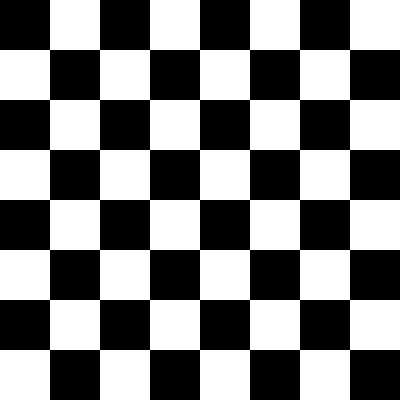
\includegraphics[scale=0.35]{checkboard.png}
			\caption{a chessboard shown by \alert{imshow(gscale(im))}}
		\end{figure}
		
		\begin{itemize}
			\item What is the image obtained from the filtering with derivatives kernels?
		\end{itemize}
	\end{exercise}
	
\end{frame}

\begin{frame}[fragile]
	
	\frametitle{First-Order derivative of image}
	\selectlanguage{english}
	\begin{itemize}
		\item Sobel and Prewitt kernel can be obtained by function \alert{\textbf{fspecial}} in Matab
		\item In Matlab, the input image should be casted to \alert{\textbf{float}} or \alert{\textbf{double}} before filtering with function \alert{\textbf{imfilter}}
	\end{itemize}
	\begin{example}
		\lstset{language=Matlab}
		\begin{lstlisting}
		clear; close all; clc;
		im = imread('cameraman.tif');
		
		H_1st_x = fspecial('Sobel');
		H_1st_y = fspecial('Sobel')'; %' = transpose
		
		im_1st_x = abs(imfilter(double(im), H_1st_x));
		im_1st_y = abs(imfilter(double(im), H_1st_y));
		
		figure, imshow(im), title('Input Image');
		figure, imshow(gscale(im_1st_x)),
		title('1st derivative on x');
		figure, imshow(gscale(im_1st_y)),
		title('1st derivative on y');
		\end{lstlisting}
	\end{example}
	
\end{frame}

\section{Gradient}
\frame
{
	\frametitle{Gradient}
	\selectlanguage{english}
	
	\begin{alertblock}{Definition}
	Gradient at a pixel in a image $f(x,y)$ is a vector $\nabla f$. It is defined as
	
	\centering
	
	$\nabla f = $ 
	$\left[ \begin{array}{r} 
		f_x \\
		f_y
	\end{array}\right]$
	
	\end{alertblock}
	

}

\frame
{
	\frametitle{Gradient}
	\selectlanguage{english}
	
	\begin{block}{Magnitude and angle of gradient vectors}
		
		\textbf{Magnitude} of gradient is computed by:
		
		$|\nabla f|=  \sqrt{f_{x}^{2} + f_{y}^{2}}$
		
		or, approximated by
		
		$|\nabla f|=  |f_{x}| + |f_{y}|$
		
		\begin{itemize}
			\item Magnitude of a gradient at pixel $(u,v)$ tells us the rate of change of intensities at $(u,v)$
			\item In other words, it tells us the edge passing $(u,v)$ is strong or not.
		\end{itemize}
		
		
	\end{block}
	
}


\frame
{
	\frametitle{Gradient}
	\selectlanguage{english}
	
	\begin{block}{Magnitude and angle of gradient vectors}
		\textbf{Angle} of gradient is computed by:
		
		$\theta(\nabla f)= $ 
		$tan^{-1}(\frac{f_{y}}{f_{x}})$
		
		\begin{itemize}
			\item Angle of a gradient at pixel $(u,v)$ tells us the orientation of edge passing $(u,v)$
			
			\item Gradient vector is perpendicular to the local edge passing $(u,v)$ 
		\end{itemize}
		
	\end{block}
	
}
\begin{frame}[fragile]
	
	\frametitle{First-Order derivative of image}
	\selectlanguage{english}
	\begin{exercise}
		\begin{figure}[!h]
			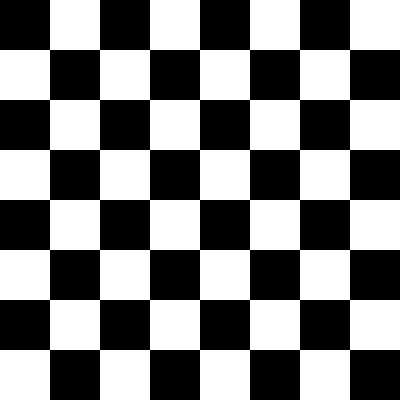
\includegraphics[scale=0.25]{checkboard.png}
			\caption{a chessboard}
		\end{figure}
		
		\begin{itemize}
			\item How do we create an image emphasizing both of horizontal and vertical edges the above chessboard?
			\item Which is the direction of gradient vectors at strong edge points?
		\end{itemize}
	\end{exercise}
	
\end{frame}

\section{Second-order derivative}
\frame
{
	\frametitle{Second-order Derivative of one variable function}
	\selectlanguage{english}
	Second-order differential can be approximated by
	
	
	\begin{align} 
		\nonumber
		f^{''}(x) \cong f^{'}(x)  - f^{'}(x+1)
	\end{align}
	
	
	First-order derivatives can be approximated as
	\begin{align}
		\nonumber 
		f^{'}(x) &\cong f(x) - f(x-1) \\
		\nonumber 
		f^{'}(x+1) &\cong f(x+1) - f(x)
	\end{align}
	
	\begin{alertblock}{Second-order derivative}
		\begin{align} 
		\nonumber
		f^{''}(x) \cong -f^{'}(x-1)  + 2f^{'}(x) - f(x+1)
		\end{align}
	\end{alertblock}
	
}
\frame
{
	\frametitle{Second-Order derivative of image}
	\selectlanguage{english}
	
	\begin{enumerate}
		\item Second-order derivative on x
		\begin{itemize}
			\item Math: 
			\begin{align}
				\nonumber
				\frac{\partial^{2} f(x,y)}{\partial x^2} = -f(x-1, y) + 2f(x,y) - f(x+1,y)
			\end{align}
			
			
			\item Kernel:  $H_{conv} = $ $\left[ \begin{array}{rrr} -1 & 2 & -1 \end{array}\right] $
			
		\end{itemize}
		\item Second-order derivative on y
		\begin{itemize}
			\item Math: 
			\begin{align}
			\nonumber
			\frac{\partial^{2} f(x,y)}{\partial y^2} = -f(x, y-1) + 2f(x,y) - f(x,y+1)
			\end{align}
			
			
			\item Kernel:  $H_{conv} = $ $\left[ \begin{array}{r} -1 \\ 2 \\ -1 \end{array}\right]$
			
		\end{itemize}
		
		
	\end{enumerate}
	
}
\frame
{
	\frametitle{Second-Order derivative of image}
	\selectlanguage{english}
	In general, second-order derivatives can be approximated by using the following kernels.
	\newline
	
	\centering
	\small
	\begin{tabular}{|l|l|l|}
		\hline
		&Derivative on x & Derivative on y \\
		\hline
		& & \\
		
		Positive at center: & 
		$H_{x} = $ $\left[ \begin{array}{rrr} -1 & 2 & -1 \end{array}\right] $ & 
		$H_{y} = $ $\left[ \begin{array}{r} -1 \\ 2 \\ -1 \end{array}\right]$\\
		
		& & \\
		\hline 
		& & \\
		
		Negative at center: & 		
		$H_{x} = $ $\left[ \begin{array}{rrr} 1 & -2 & 1 \end{array}\right] $ &
		$H_{y} = $ $\left[ \begin{array}{r} 1 \\ -2 \\ 1 \end{array}\right]$\\
		& & \\
		
		\hline 
	\end{tabular}
}

\frame
{
	\frametitle{First-order and Second-order derivative}
	\selectlanguage{english}
	\begin{figure}[!h]
		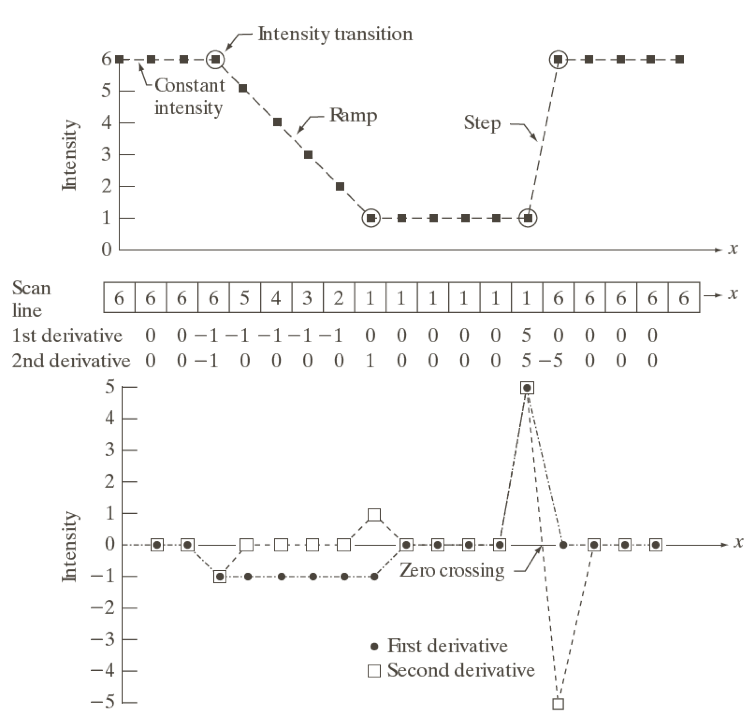
\includegraphics[scale=0.6]{derivatives.png}
		\caption{Example of First-order and Second-order derivatives }
	\end{figure}
}

\frame
{
	\frametitle{First-order and Second-order derivative}
	\selectlanguage{english}
	\begin{alertblock}{First-order derivative's properties}
		\begin{enumerate}
			\item First-order derivatives produce \alert{\textbf{thicker edge}} in an image.
			\item First-order derivatives produce \alert{\textbf{strong response}} to a gray-level step.
			
		\end{enumerate}
		
	\end{alertblock}
	
	\begin{alertblock}{Second-order derivative's properties}
		\begin{enumerate}
			\item Second-order derivatives produce \alert{\textbf{stronger response}} to fine detail, such as thin lines or isolated points (noise).
			\item Second-order derivatives produce \alert{\textbf{double response}} (a \alert{\textbf{positive}} and a \alert{\textbf{negative}}) at step change in in gray level.
			\item \alert{\textbf{Zero-crossing}} at a point in second-order derivatives indicates that there is an edge passing that point.
			
		\end{enumerate}
		
	\end{alertblock}
}

\section{Laplacian}
\frame
{
	\frametitle{Second-Order derivative of image}
	\selectlanguage{english}
	
	\alert{\textbf{Second-order derivative on x and y}}
	
	Laplacian operator: 
	\begin{align}
		\nonumber
		\nabla^{2}f = \frac{\partial^{2} f(x,y)}{\partial x^2}  + \frac{\partial^{2} f(x,y)}{\partial y^2} 
	\end{align}
	
	\begin{itemize}
		\item Math: 
		\begin{align}
		\nonumber
		\nabla^{2}f & = &-f(x-1, y) + 2f(x,y) - f(x+1,y) \\
		\nonumber
		&&-f(x, y-1) + 2f(x,y) - f(x,y+1)
		\end{align}
		
		
		\item Kernel:  $H_{lap} = $ $\left[ 
		\begin{array}{rrr} 
		0 & -1 & 0 \\
		-1 & 4 & -1\\
		0 & -1 & 0
		\end{array}\right] $
		
	\end{itemize}
	
	
}
\frame
{
	\frametitle{Second-Order derivative of image}
	\selectlanguage{english}
	
	\alert{\textbf{Second-order derivative on x, y, and diagonals:}}
	
	Extended Laplacian operator: 
	
	\begin{itemize}
		\item Math: 
		\begin{align}
		\nonumber
		\nabla^{2}f & = &-f(x-1, y) + 2f(x,y) - f(x+1,y) \\
		\nonumber
		&&-f(x, y-1) + 2f(x,y) - f(x,y+1)
		\end{align}
		
		
		\item Kernel:  $H_{lap} = $ $\left[ 
		\begin{array}{rrr} 
		-1 & -1 & -1 \\
		-1 & 8 & -1\\
		-1 & -1 & -1
		\end{array}\right] $
		
	\end{itemize}
}

\frame
{
	\frametitle{Second-Order derivative of image}
	\selectlanguage{english}
	
	In general, Laplician can be computed by using the following kernels. The center coefficients maybe positive or negative.
	\newline
	
	\centering
	\begin{tabular}{|l||l|}
		\hline
		& \\
		$H_{lap} = $ $\left[ 
		\begin{array}{rrr} 
		0 & -1 & 0 \\
		-1 & 4 & -1\\
		0 & -1 & 0
		\end{array}\right] $ 
		&
		$H_{lap} = $ $\left[ 
		\begin{array}{rrr} 
		-1 & -1 & -1 \\
		-1 & 8 & -1\\
		-1 & -1 & -1
		\end{array}\right] $ \\
		& \\
		\hline
		& \\
		$H_{lap} = $ $\left[ 
		\begin{array}{rrr} 
		0 & 1 & 0 \\
		1 & -4 & 1\\
		0 & 1 & 0
		\end{array}\right] $ 
		&
		$H_{lap} = $ $\left[ 
		\begin{array}{rrr} 
		1 & 1 & 1 \\
		1 & -8 & 1\\
		1 & 1 & 1
		\end{array}\right] $ \\
		& \\
		\hline
	\end{tabular}

	
	
}
\section{Applications of Laplacican}
\frame
{
	\frametitle{Applications of Laplacican operator}
	\begin{alertblock}{Properties of Laplacican operators}
		\begin{enumerate}
			\item \textbf{Highlight} gray-level discontinues in images, i.e., edges on images
			\item \textbf{De-emphasize} regions with slowly varying gray-levels
		\end{enumerate}
		
		Therefore, adding (or subtracting) the original image with Laplacian image (the image obtained by filtering the original with Laplacian kernel) $\Rightarrow$ \alert{\textbf{Sharpened images}}
	\end{alertblock}
	
}
\frame
{
	\frametitle{Applications of Laplacican operator}
	Method for sharpening  image $f(x,y)$:
	\flushleft
	$$
	g(x,y) =
	\begin{cases}
		f(x,y) - \nabla^2f(x,y)& 	\text{if the center coefficient of the}\\
			& \text{Laplacian mask is negative }\\
		f(x,y) + \nabla^2f(x,y)& 	\text{if the center coefficient of the} \\
		&  \text{Laplacian mask is positive }
	\end{cases}
	$$
	
}
\frame
{
	\frametitle{Second-Order derivative of image}
	\selectlanguage{english}
	Method for sharpening  image $f(x,y)$ by using linear filters. Kernels are as follows:
	\newline
	
	\begin{tabular}{|l|l|}
		\hline
		\textbf{Positive central coefficient} & \textbf{Positive central coefficient} \\
		\hline
			& \\
			$H_{Lap} = $ $\left[ 
			\begin{array}{rrr} 
			-1 & -1 & -1 \\
			-1 & 9 & -1\\
			-1 & -1 & -1
			\end{array}\right] $ &
			$H_{Lap} = $ $\left[ 
			\begin{array}{rrr} 
			1 & 1 & 1 \\
			1 & -9 & 1\\
			1 & -1 & 1
			\end{array}\right] $ \\
			& \\
		\hline
			& \\
			$H_{Lap} = $ $\left[ 
			\begin{array}{rrr} 
			0 & -1 & 0 \\
			-1 & 5 & -1\\
			0 & -1 & 0
			\end{array}\right] $ &
			$H_{Lap} = $ $\left[ 
			\begin{array}{rrr} 
			0 & 1 & 0 \\
			1 & -5 & 1\\
			0 & -1 & 0
			\end{array}\right] $ \\
			& \\
			\hline
	\end{tabular}

	
	
}
\frame
{
	\frametitle{Applications of Laplacican operator: Examples}
	\selectlanguage{english}
	\begin{figure}[!h]
		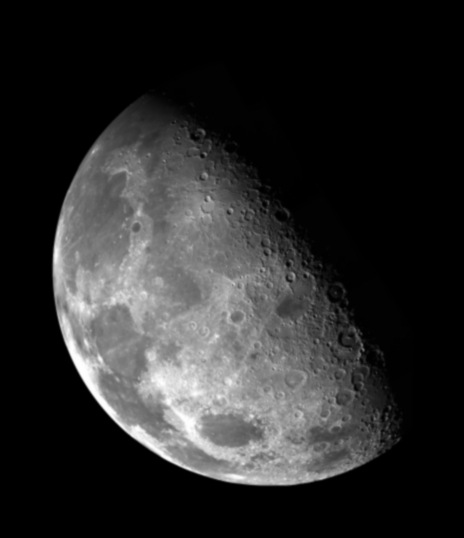
\includegraphics[scale=0.4]{north_pole.jpg}
		\caption{Input image: North pole of moon}
	\end{figure}	
}
\frame
{
	\frametitle{Applications of Laplacican operator: Examples}
	\selectlanguage{english}
	\begin{figure}[!h]
		\begin{tabular}{cc}
			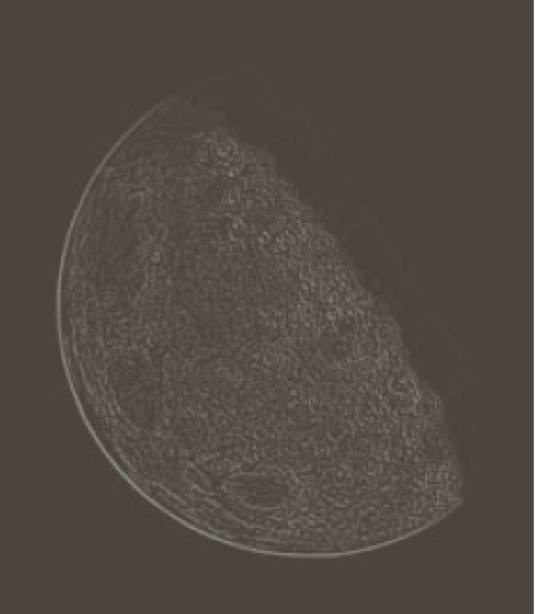
\includegraphics[scale=0.5]{north_pole_laplacian_unscaled.png} &
			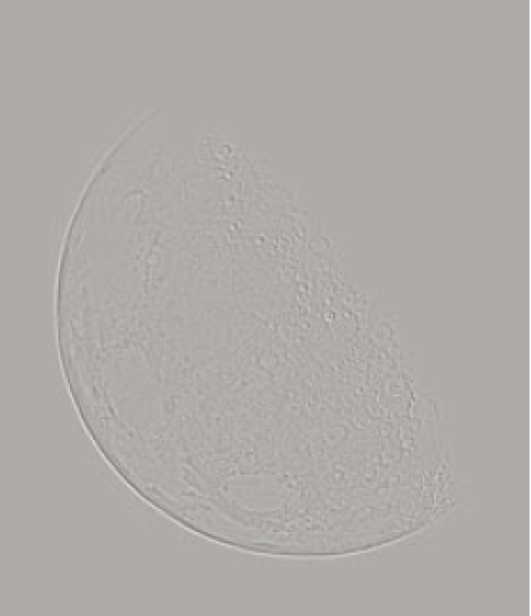
\includegraphics[scale=0.5]{north_pole_laplacian_scaled.png} \\
			(a) & (b)
		\end{tabular}
		\centering
		\caption{Laplacian images = images obtained by filtering with Laplacian operator: (a) without scaling, (b) with scaling for display purpose}
	\end{figure}	
}
\frame
{
	\frametitle{Applications of Laplacican operator: Exercises}
	\selectlanguage{english}
	\begin{exercise}
		\begin{enumerate}
			\item How can you sharpen images, e.g., north pole of moon, with Laplacian by using Matlab and OpenCV?
			\item Create blurred version and then sharpen the blurred version
			\begin{itemize}
				\item Read checkboard image from file
				\item Blur it with Box or Gaussian filter
				\item Sharpen the resulting blurred version with Laplacian
				\item Show the original, blurred version and sharpened version.
			\end{itemize}
		\end{enumerate}
		
	\end{exercise}	
}

\frame
{
	\frametitle{Unsharp masking and High-boost filtering}
	\selectlanguage{english}
	\textbf{Unsharp masking:}  image obtained from subtracting a blurred version of an image from the image itself.
	
	\begin{align}
		\nonumber
		f_s(x,y) &= f(x,y) - \bar{f}(x,y)
	\end{align}
	\begin{itemize}
		\item $\bar{f}(x,y)$ : blurred version of $f(x,y)$, e.g., using box filter
		\item $f_s(x,y)$: sharpened image
	\end{itemize}
}
\frame
{
	\frametitle{Unsharp masking and High-boost filtering}
	\selectlanguage{english}
	\begin{exercise}
		\begin{enumerate}
			\item How can you implement unsharp masking with Matlab and OpenCV?
			\item Create blurred version and then sharpen the blurred version
			\begin{itemize}
				\item Read checkboard image from file
				\item Blur it with Box or Gaussian filter
				\item Sharpen the resulting blurred version with Unsharp masking
				\item Show the original, blurred version and sharpened version.
			\end{itemize}
		\end{enumerate}
		
	\end{exercise}
}

\frame
{
	\frametitle{Unsharp masking and High-boost filtering}
	\selectlanguage{english}
	\textbf{High-boost filtering:}  a generalized unsharpened image.
	
	\begin{align}
	\nonumber
	f_{hb}(x,y) &= Af(x,y) - \bar{f}(x,y)
	\end{align}
	\begin{itemize}
		\item $A$ : a parameter, $A \ge 1$. $A=1$, hight-boost filtering $\rightarrow$ unsharp masking
		\item $f_s(x,y)$: sharpened image
	\end{itemize}
}
\frame
{
	\frametitle{Unsharp masking and High-boost filtering}
	\selectlanguage{english}
	\textbf{High-boost filtering:}  Other representations.
	
	\begin{align}
	\nonumber
	f_{hb}(x,y) &= Af(x,y) - \bar{f}(x,y)\\
	\nonumber
				&= (A-1)f(x,y) + f(x,y) - \bar{f}(x,y)\\
				&= (A-1)f(x,y)  + f_s(x,y) \label{eq:hb_filter}
	\end{align}
	Replace Eq. (\ref{eq:hb_filter}) with Laplacian sharpening filter:
	\small
	$$
	f_{hb}(x,y) =
	\begin{cases}
	Af(x,y) - \nabla^2f(x,y)& 	\text{if the center coefficient of the}\\
	& \text{Laplacian mask is negative }\\
	Af(x,y) + \nabla^2f(x,y)& 	\text{if the center coefficient of the} \\
	&  \text{Laplacian mask is positive }
	\end{cases}
	$$
	
}
\frame
{
	\frametitle{Unsharp masking and High-boost filtering}
	\selectlanguage{english}
	\textbf{High-boost filtering:}  can be implemented as a linear filter, with one of the following kernels.
	\newline
		\newline
	\centering
	\begin{tabular}{l||l}
		 \\
		$H_{hb8} = $ $\left[ 
		\begin{array}{rrr} 
		-1 & -1 & -1 \\
		-1 & A+8 & -1\\
		-1 & -1 & -1
		\end{array}\right] $ &
		$H_{hb4} = $ $\left[ 
		\begin{array}{rrr} 
		0 & -1 & 0 \\
		-1 & A+4 & -1\\
		0 & -1 & 0
		\end{array}\right] $ \\
		\\
	\end{tabular}
	\flushleft
	\textbf{$A$ is a parameter:}
	\begin{enumerate}
		\item  $A=0$, hight-boost filter becomes standard \alert{Laplacian filter}
		\item  $A=1$, hight-boost filter becomes standard \alert{Laplacian sharpening filter}
		\item $A$ increases pass $1$ the contribution of sharpening process becomes less and less important
	\end{enumerate}
}
\frame
{
	\frametitle{Unsharp masking and High-boost filtering}
	\selectlanguage{english}
	\begin{alertblock}{Applications of High-boost filtering:}
		\begin{itemize}
			\item  High-boost filtering can sharpen images
			\item  High-boost filtering can brighten dark images
		\end{itemize}
		
	\end{alertblock}	
}
\frame
{
	\frametitle{Unsharp masking and High-boost filtering: Examples}
	\selectlanguage{english}
	\begin{figure}[!h]
		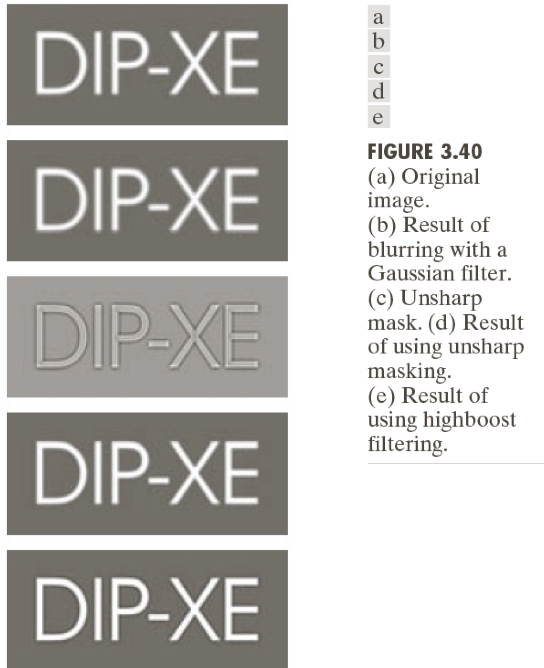
\includegraphics[scale=0.75]{highboost.png}
	\end{figure}	
}
%%%%%%%%%%%%%%%%%%%%%%%%%%%%%%%%%%%%%%%%%%%%%%%

%%%%%%%%%%%%%%%%%%%%%%%%%%%%%%%%%%%%%%%%%%%%%%%

\end{document}